\documentclass[conference,compsoc]{IEEEtran}
\usepackage{ifpdf}
\usepackage{caption}
\usepackage[pdftex]{graphicx}
\usepackage[noadjust]{cite}
\usepackage{amsmath}
\usepackage[caption=false,font=footnotesize,labelfont=sf,textfont=sf]{subfig}
\usepackage{fixltx2e}
\hyphenation{op-tical net-works semi-conduc-tor}
\renewcommand{\citedash}{--}


\begin{document}

\title{Visual Dataflow Language for Educational Robots Programming}

\author{
	\IEEEauthorblockN{Grogorii Zimin}
	\IEEEauthorblockA{
		Mathematics and Mechanics Faculty,\\
		SPbSU\\
		Saint-Petersburg, Russia \\
		Email: zimin.grigory@gmail.com
	}
	
	\and

	\IEEEauthorblockN{Dmitrii Mordvinov}
	\IEEEauthorblockA{
		Mathematics and Mechanics Faculty,\\
		SPbSU\\
		Saint-Petersburg, Russia \\
		Email: mordvinov.dmitry@gmail.com
	}
}

\maketitle



\begin{abstract}
REWRITE THIS SH..
The paper describes dataflow visual programming language based on DSM-approach. Its purpose is to be bridge between lightweight robotics languages for education and complex industrial languages. A short review of programming languages for robots is presented here. Also different approaches and architectures for developing control system for robots are considered. For demonstration of language usage, the paper provide solution for creating control system of robot based on subsumption architecture. 
\end{abstract}

\section{Introduction}

Programming languages for creating robotic controllers are actual topics of research oftenly discussed at major conferences, such as ICRA\cite{Icra} or IROS\cite{Iros2016}. Visual programming languages (VPLs) are also actively discussed for the last three decades, the largest conferences are held annually, e.g. VL/HCC\cite{VLHCC}. VPLs are oftenly applied in robotics domain\cite{banyasad2000visual,simpson2006mobile,simpson2008visual,posso2011process,diprose2011ruru} allowing to create and visualize robotic controllers. Robotic VPLs are commonly used for educational purposes, making possible for students of even junior schools to create robotic programs. There already exists a great number of educational robotic programming environments based on VPLs, e.g. NXT-G\cite{nxtg}, TRIK Studio\cite{trik}, ROBOLAB\cite{robolab}, also there are some academic tools implementing interesting and novel approaches to educational robotics programming\cite{banyasad2000visual,simpson2008visual,diprose2011ruru}.

Robotic control programs are inherently reactive: they transform data which is continuously coming from multiple sensors into the impulses on actuators. For this reason dataflow languages (DFLs) are well-suitable for robotics programming. Many researchers denoted the conveniency of dataflow visual programming languages (DFVPLs)\cite{johnston2004advances}, finding them more useful than textual DFLs, for example because data flows explicitly displayed on the diagram. There are large and complex general-purpose and domain-specific development environments such as LabVIEW\cite{labview} and Simulink\cite{simulink} that provide a large (and sometimes even cumbersome) set of libraries for robotics programming. More detailed discussion of robotics VPLs will be provided in section~\ref{sec:Overview}.

There is a large number of robotic constructor kits for learning the basics of robotics and cybernetics, such as LEGO MINDSTORMS\cite{legokit}, TRIK, ScratchDuino\cite{http://www.scratchduino.com/}. Modern programming languages that are used for programming those kits are based on the control flow model rather than on dataflow model. Control flow-based languages are good for solving scholar ``toy'' tasks, but may be inconvenient for programming more complex ``real world'' controllers that may be conveniently expresses on DFLs. The simple DFVPL may be considered as a useful step from educational VPLs to the programming languages that are used in unversities and industry. 

This paper discusses a novel extensible tool for programming all popular educational robotic kits on dataflow visual programming language. One of the most important distinction of our tool from others is its focus on embedded systems (sec.~\ref{sec:Implementation}). Another interesting detail of our work is the application of DSM-aproach for implementation of visual editor: it is entirely generated by QReal DSM-platform\cite{qrealMeta}\cite{kuzenkova2013qreal} without even a line of code written. We also take into consideration the popularity of Brooks' Subsumption Architecture\cite{brooks1986robust} which is still mainstream aproach to design of complex robotic controllers\cite{banyasad2000visual,simpson2006mobile,posso2011process,proetzsch2007behaviour} despite it was proposed 30 years ago. Brooks’ Subsumption Architecture and some other are conveniently expressed in our language, they are discussed in sec.~\ref{}.

The remainder of a paper is organized as follows. An overview of robotics VPLs and DFVPLs is presented in section~\ref{sec:Overview}. A description of our language is given in section~\ref{sec:lang}. Section~\ref{sec:example} demonstrates two typical robotic controllers expressed in our language. The most important details of implementation are deiscussed in section~\ref{sec:Implementation}. Finally, the last section concludes the paper and discusses possible directions for future work.


\section{Similar Tools}
\label{sec:Overview}
Robot programming environments can be divided into three categories: educational, which allows to program small educational robotic kits; industrial, which have a rich toolkit for creating large and complex robotic controllers; academic, which implement new interesting ideas, however they are oftenly unavailable for downloading or unusable.

Educational visual enviroments are for example NXT-G and ROBOLAB for LEGO MINDSTORMS NXT kit, EV3 Software for the Lego Mindstorms EV3 kit, TRIK Studio for NXT, EV3 and TRIK. Those environments simplify solving primitive robot control tasks like finding a way out of the maze and driving along the line using light sensors, which makes the process of learning the basics of programming and robot control easy. But their simplicity oftenly bounds the flexibility of the language. Visual languages of all mentioned systems are based on control flow model.

There is also a number of well-known visual robotic programming environments of industrial level. For example, general-purpose LabVIEW from National Instruments with the DFVPL G, programming environment Simulink developed by MathWorks for modeling different dynamic models or control systems. Those products offer to a huge set of models and libraries to create control systems, test benches, real-time systems of any complexity, using model-driven approach. LabVIEW provides opportunity for programming small robots. There are lots of examples of applying LabVIEW in education\cite{erwin2000lego, 1_gomez-de-gabriel_mandow_fernandez-lozano_garcia-cerezo_2011}, but much more oftenly its adaptations like Robolab are used in educational process. It should be noted that those environments are distributed under the commercial license.

Another example of an visual robotics industrial system is the Microsoft Robotics Developer Studio (MSRDS)\cite{jackson2007microsoft}, which is free for academic purposes and allow to create distributed robotic systems on DFVPL. MSRDS officially supports a large set of robotic platforms, LEGO NXT\cite{kim2007programming} in particular (however, the autonomious mode for NXT is not supported). MSRDS has the ability of manual integration with custom robotic platforms, but unhappily is not maintained since 2014.

There is a lot of scientific research done in this area, e.g., dissertation\cite{banyasad2000visual} describes a visual programming module for expressing robotic controllers in terms of extended Moore machines, \cite{simpson2008visual},\cite{posso2011process} describe visual environment for $occam\mbox{-}\pi$ language and $Transterpreter$ framework, and its usage in education and swarm robotics. Article\cite{diprose2011ruru} describes DFVPL for beginners which is pretty close to a one we introduce here. However at the moment RuRu is under development, it has pretty limited functionality and even unavailable for download.

% Нужна секция с архитектурами! Не забыть дополнить конец введения!
%There are several commonly used robots controller architectures: Connell's Colony, Maes' Action-Selection, Arkin's Motor Schema, Rosenblatt's Distributed Architecture for Mobile Navigation, Brooks' Subsumption Architecture\cite{simpson2009toward}. 

\section{Description of the Language}
\label{sec:lang}
Evolution of a domain-specific modeling (DSM) methodology allows to quickly create a fairly sophisticated visual programming languages\cite{DSM}.

%Развитие модельно-ориентированного подхода\cite{koznov2008} позволило быстро создавать достаточно сложные визуальные языки программирования. Среда программирования TRIK Studio является примером системы, созданной с применением DSM-подхода на базе платформы QReal\cite{qrealMeta}\cite{kuzenkova2013qreal}. Основываясь на промышленном опыте разработчиков TRIK Studio, было решено создавать потоковый язык программирования роботов на базе платформы QReal. Первый прототип языка был создан в течение недели. На момент написания статьи язык и средства его поддержки находятся в активной разработке. Опишем некоторые особенности разрабатываемой технологии.

%\begin{itemize}
%\item Архитектура Брукса легко выражается средствами языка.
%\item Диаграммы поведения роботов, так же как и в TRIK Studio, имеют возможность быть проинтерпретированными на двумерной имитационной модели робота. 
%\item В ближайших планах стоит генерация диаграмм потоков данных в текстовые языки, используемые для программирования TRIK --- в первую очередь, JavaScript, F\#\cite{kirsanov2014robotics} и Kotlin.
%\end{itemize}

%\section*{Элементы языка}
%Элементы языка можно разделить по назначению на несколько групп.

%\begin{itemize}
%\item \textit{Элемент потока данных}. Связь, реализующая поток для передачи данных. 
%\item \textit{Блоки управления приводами}. Блоки принимающие числовые значения, отвечающие за подачу импульсов на приводы (силовые моторы, сервомоторы и т.д.).
%\item \textit{Блоки считывания данных с сенсоров}. Блоки, генерирующие соответствующие значения, которые подлежат дальнейшей обработке.
%\item \textit{Блоки синхронизации и фильтрации}. Позволяют временно блокировать передачу данных, устанавливать количество наборов пропускаемых данных и время между отправками. 
%\item \textit{Блоки поддержки устройств ввода}. Считывают данные с устройств операторского контроля (в данный момент поддержан только джойстик, в планах --- компьютерная мышь и клавиатура). 
%\item \textit{Блоки рисования на экране}. Отвечают за векторное и растровое рисование на экране.
%\item \textit{Блоки видеозрения}. Предоставляют доступ ко всем возможностям видеозрения контроллера TRIK.
%\item \textit{Блоки взаимодействия между роботами}. Отвечают за групповую координацию роботов.
%\item \textit{Блок текстового программирования}. Блок, позволяющий произвести обработку входных данных на текстовом языке (статически типизируемом диалекте Lua, поддержка которого <<унаследована>> от кодовой базы TRIK Studio). Чаще всего такой блок будет использоваться для задания математических операций над данными.
%\item \textit{Блоки управляющих конструкций}. Включают циклы, условные развилки, множественный выбор, распараллеливание, подавление и ингибицию, блок <<Подпрограмма>> для переиспользования кода. Последние четыре блока обеспечивают поддержку архитектуры Брукса в языке.

%\end{itemize} 

\section{Example}
\label{sec:example}

%Рассмотрим задачу управления движением робота при помощи джойстика, при условии, что робот сам избегает лобовых столкновений с припятствиями. Предполагается, что программа пишется для двухколесного мобильного робота, оборудованного спереди инфракрасными датчиками расстояния, для управления колесами используются силовые моторы.

%Разобьем задачу на два уровня поведения. Первый будет отвечать за обслуживание запросов пользователя. Второй будет ответственен за избегание столкновений: если робот близок к столкновению, то он должен уклониться от препятствия вне зависимости от того, что нажимает пользователь на пульте. 

%Рассмотрим первый уровень (рис.~\ref{image:layer1}). Пользователь управляет роботом посредством джойстика. Джойстик генерирует данные, соответствующие нажатиям кнопок или манипулирований рычагом направления. Для простоты считаем, что нажатие любой кнопки завершит программу управления роботом. Данные с рычага преобразуются блоком текстового программирования в соответствующие импульсы моторов робота, которые в данном случае передаются <<заглушкам>>, которые связаны с выходными портами блока <<Подпрограмма>>. 
%\begin{figure}[ht]
%	\centering
%	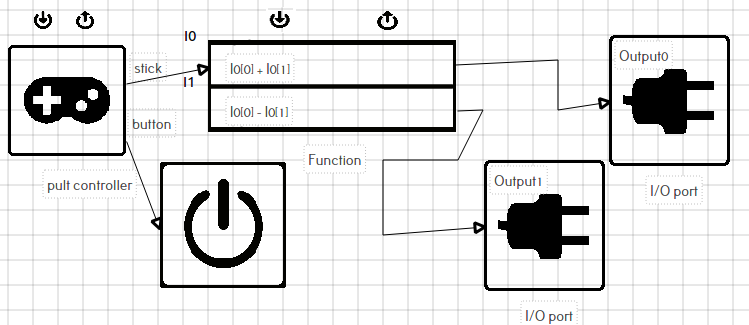
\includegraphics[width=3.5in]{pultLayer.png}
%	\caption{Уровень управления с пульта.}
%	\label{image:layer1}
%\end{figure}

%Рассмотрим второй уровень (рис.~\ref{image:layer2}): данные с датчиков расстояния собираются в вектор и передаются фильтру, который при опасности столкновения отправляет данные дальше в блок математической обработки (если условие не выполнилось, управление может быть передано по потоку <<ошибки>>, в данной программе этот поток не указан; также между проверками условия приходящие данные не обрабатываются (теряются) в течение установленного пользователем времени). В блоке математической обработки вычисляется мощность, которую необходимо подать на 2 мотора. Вычисленные значения передаются выходным портам.
%\begin{figure}[ht]
%	\centering
%	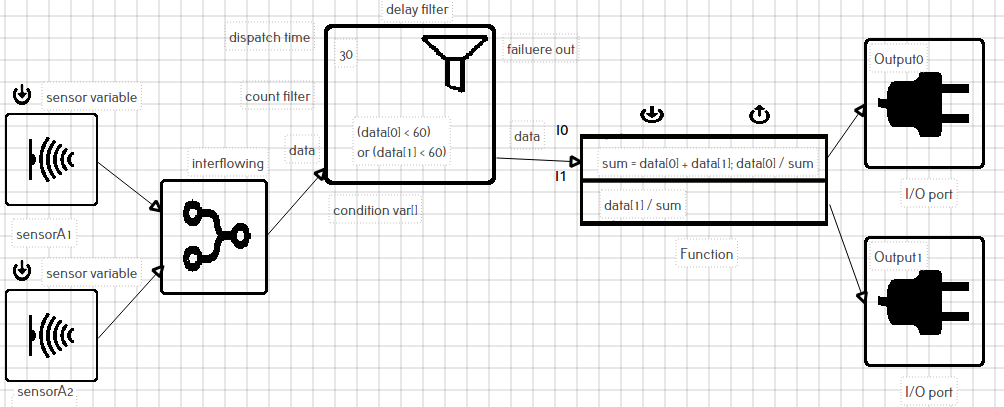
\includegraphics[width=3.5in]{collisionLayer.png}
%	\caption{Уровень избегания столкновений.}
%	\label{image:layer2}
%\end{figure}

%\begin{figure}[ht]
%	\centering
%	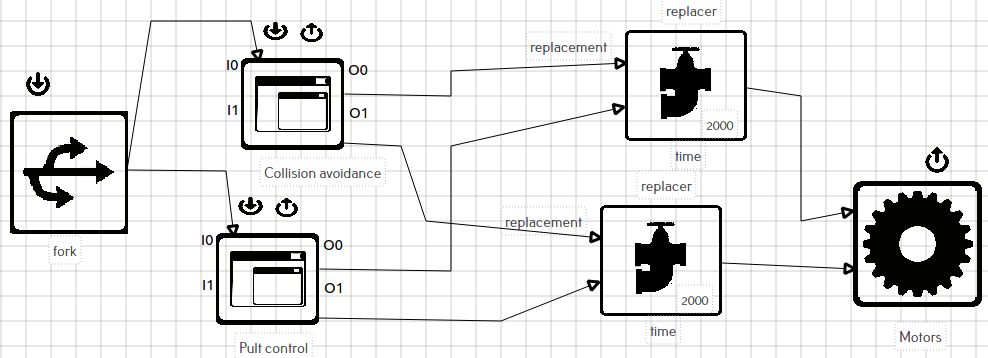
\includegraphics[width=3.5in]{programScreen.png}
%	\caption{Программа управления роботом.}
%	\label{image:prog}
%\end{figure}

%Имея два поведения, создаем управление роботом в модели Брукса (рис.~\ref{image:prog}). С помощью блока распараллеливания запускаем уровни поведения. Каждый уровень генерирует данные, соответствующие мощностям моторов, передаваемые на блок управления силовыми моторами. Так как второй уровень ответственности должен не позволить столкнуться с препятствием, его значения подавляют значения, полученные с первого уровня, с помощью блоков <<Подавления>>.

\section{Implementation}
\label{sec:Implementation}
The system is implemented as two plugins for TRIK Studio. The first one describes the visual language and provides visual editor for our system. It contains the metamodel of dataflow visual language and entirely generated by QReal DSM-platform. Plugged into TRIK Studio this module provides fully operational visual editor with all advantages of TRIK Studio control flow editor like modern-looking user interface, ability to create elements with mouse gestures, different appearances of links and so on. The time spent on the development of this plugin (not considering discussing and designing the prototype of visual language on paper) roughly equals three man-days. The benefit on exploiting the DSM-aproach is obviuos, the development of the similar editor from scratch would have been taken vastly more time.

The second plugin contains implementation of dataflow diagrams interpreter. Given the program drawn in editor (provided by first plugin) interpreter will transform that program into a sequence of the commands sent to a target robot (see fig.~\ref{image:common-architecture}). The target robot can be one of the supported in TRIK Studio infrasctructure: Lego NXT or EV3 robot, TRIK robot, TRIK Studio 2D simulator or $V\mbox{-}REP$ 3D simulator\cite{rohmer2013v}. Commands are sent via high-level TRIK Studio devices API, a part of it presented at fig.~\ref{image:devices-architecture}.

\begin{figure}[ht]
	\centering
	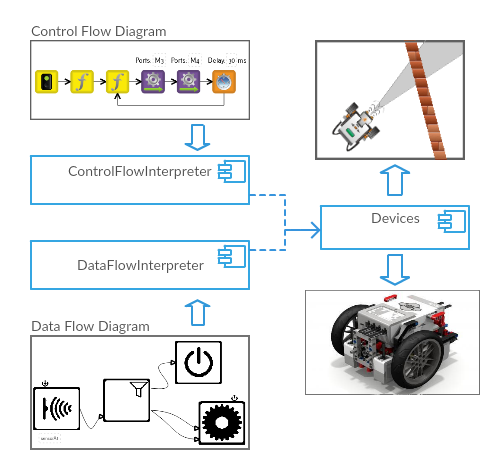
\includegraphics[width=3.5in]{Common.png}
	\caption{The general acrhitecture of the system}
	\label{image:common-architecture}
\end{figure}

\begin{figure}[ht]
	\centering
	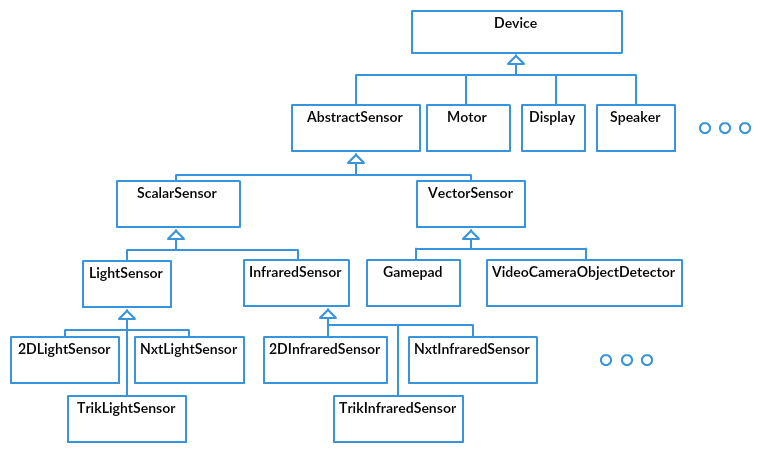
\includegraphics[width=3.5in]{Devices.png}
	\caption{Partial architecture of devices used in dataflow interpreter}
	\label{image:devices-architecture}
\end{figure}

The general acrhitecture of intepreter plugin is presented at fig.~\ref{image:interpreter-architecture}. Given dataflow diagram interpreter traverses, validates and prepares it for interpretation process. For each visited dataflow block implementation object is instantiated. Implementation objects are written in c++. Instantiation is performed by corresponding factory object. Implementation objects are then subscribed each to other like they are connected by flows on diagram, \textit{publish-subscribe} pattern is used here. The set of initial blocks is determined next, those are blocks without incomming flows. After all that done preparation phase is complete and diagram starts beeing interpreted.

\begin{figure}[ht]
	\centering
	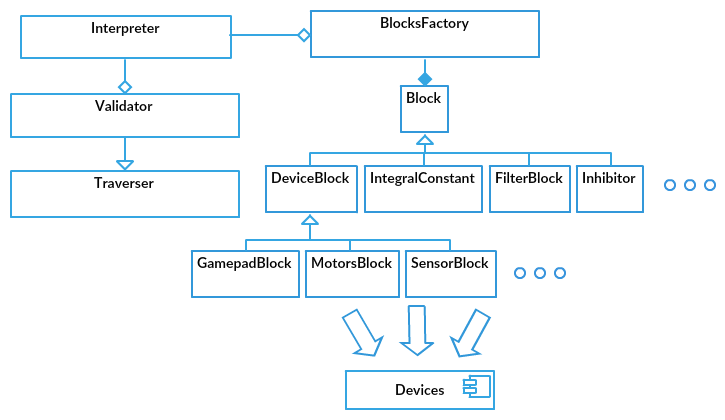
\includegraphics[width=3.5in]{Interpreter.png}
	\caption{The general architecture of dataflow interpreter plugin}
	\label{image:interpreter-architecture}
\end{figure}

Interpretation process is not as straightforward as in most asynchronious dataflow environments. Usually components of dataflow diagram are executed concurrently, on differents threads, processes or even machines (that is actively exploited, for example, by Microsoft Robotics Developer Studio where dataflow diagram is deployed into a number of web-services). That is a pretty convenient way to invoke dataflow diagrams on a powerful hardware, but not a case when we talk about embedded devices. In out case we deal exactly with embedded devices (Lego NXT, EV3, TRIK, Arduino controllers), so we propose here another way of executing dataflow diagrams. The main idea is to intoduce global message queue and event loop for messages processing. When token is published by some block it is enqueued into messages queue and waits for its turn to be delivered to subscribers (fig.~\ref{image:interpreter-interaction}). In fact thus we \textit{flatten} the execution, convert concurrent way of dataflow interpretation to a pseudo-concurrent one where we schedule invocation order on our own. It must be noted that this mechanism is similar to events propagation system of Qt framework. That is actively exploited in our implementation, where message processing is completely performed by $QEventLoop$ class and tokens delivering is done by Qt signal/slot system in $QueuedConnection$ mode. 

Flat execution of dataflow diagram poses a number of small problems, one of them will be discussed here. Input device blocks (for example blocks publishing tokens from ultrasonic sensors) are constantly emitting tokens to subscribers. Subscribers transmit tokens to a next one (possibly in modified state) and so on. Thus there appears a chain of data processing. In out language that chain can activate control flow ports of blocks ``reviving'' them, so the control flow model is implicitly supported in out language (this is important in educational reasons). If later in this chain same input device block will be met then execution will come in a 
counterintuitive way. Such conflicts are ruled out with a simple heruistic that among all the blocks sharing one physical device only one can be active and that is the last activated one. Thus when the execution token comes into some device block it immediately ``deactivates'' conflicting ones. Other problems like messages balancing (in case when some block ``flooding'' the whole messages queue) will not be discussed here.

The last thing we should remark here is the presence of $Fork$ block in our language that usually is not provided by dataflow languages. Flattened model seems to work well on embedded devices, but sometimes users still need to use concurrent execution (for example for executing layers in subsumption architecture). For that reason $Fork$ block is introduced, it forks the execution into a number of platform-specific execution units (for example $pthreads$ on UNIX or $tasks$ on NXT OSEK). This block can be ragarded as low-level control of execution process. It should be also marked that this block almost has no sence in interpretation mode (because execution itself is performed on desktop machine with only sending primitive commands to robot), but will be very useful in future works when autonomous mode will be introduced.

\begin{figure}[ht]
	\centering
	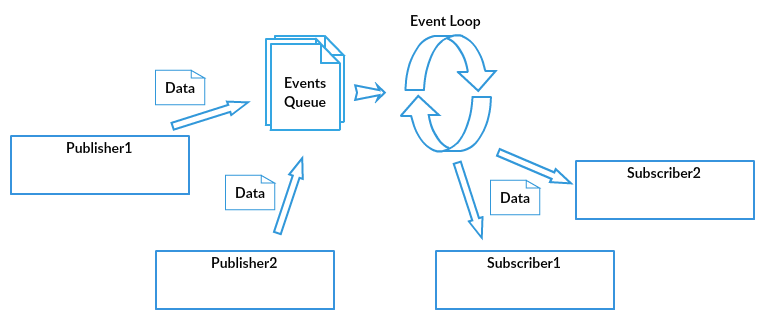
\includegraphics[width=3.5in]{Interaction.png}
	\caption{Proposed mechanism of pseudo-concurrent dataflow interpretation}
	\label{image:interpreter-interaction}
\end{figure}


\section{Conclusion and Discussion}
\label{sec:Conclusion}
In this work we presented the prototype of dataflow language for programming different robotic kits (LEGO MINDSTORMS NXT, LEGO MINDSTORMS EV3, TRIK). The system provides ability to interpret diagrams on 2D- an 3D-simulators and real robotic devices. Proposed an aproach for executing dataflow diagrams on embedded devices. The language implicitly supports control flow model for educational purposes. It is also convenient for expressing typical robotic controllers architectures which is demostrated on example.

The implemented system can be regarded as a platform for future investigations. First of all autonomious mode of work will be implemented. That will be done through code generation into a number of textual languages aready supported by TRIK Studio (NXT OSEK C for Lego, bytecode for EV3, JavaScript, F\#\cite{kirsanov2014robotics} and Kotlin for TRIK). We are also interested in academical research. First of all a formal semantics of our language should be expressed for applying various formal methods of program analysis. Another branch of research will be directed into a DSM-branch, here we want to consider an ability of dynamic langiage metamodel generation from specifications of available modules of robotics middleware (like ROS\cite{quigley2009ros} or Player\cite{gerkey2003player}).

\newpage
\bibliography{IEEEbibl}
\bibliographystyle{IEEEtran}
\end{document}
